\documentclass{standalone}
\usepackage{pgfplots}
\usetikzlibrary{arrows.meta}
\pgfplotsset{compat=newest}
\begin{document}
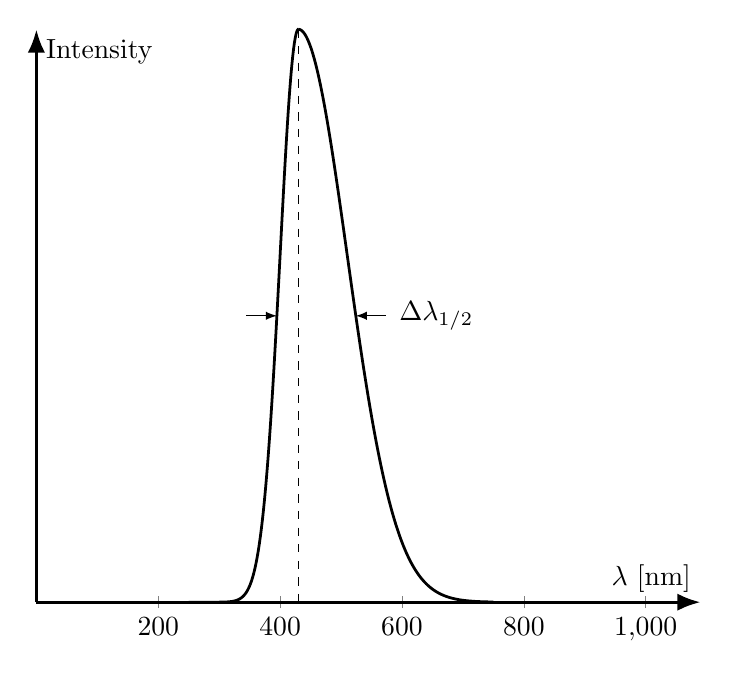
\begin{tikzpicture}
\begin{axis}[
axis lines=center,
ytick=\empty,
xlabel={$\lambda$ [nm]},
ylabel={Intensity},
xmin=0,xmax=1090,
xmajorgrids=false,
clip=false,
inner axis line style={-Latex,very thick},
scale only axis=true,
%height=200pt,
%width=400pt,
]
\addplot[line width=1pt,samples=300,domain=250:430]
{exp(-(x-430)^2/(2*30^2))};
\addplot[line width=1pt,samples=300,domain=430:750]
{exp(-(x-430)^2/(2*80^2))};
\draw[latex-] (axis cs:394.67,0.5) -- +(-50,0);
\draw[latex-] (axis cs:524.19,0.5) -- node[right]{$\ \ \Delta \lambda_{1/2}$} +(50,0);
\draw [dashed] (axis cs:430,1) -- +(0,-1);
\end{axis}
\end{tikzpicture}
\end{document}